\subsection{Statechart}
    \begin{flushleft}
        Gli statechart sono uno strumento
        di modellazione grafica, utile per rappresentare il funzionamento di un
        sistema. Sono caratterizzati da stati e transizioni, che rappresentano il
        passaggio tra stati diversi. Sono inoltre molto importanti poichè forniscono
        un chiaro mezzo di costruzione di prototipi statici: con pochi semplici
        simboli è possibile modellare l'intero funzionamento di un'interfaccia grafica.
        Useremo questo potente strumento per rappresentare i seguenti casi d'uso:
        \emph{\textbf{Aggiungi ristorante}}, \emph{\textbf{Aggiungi piatto}}, 
        \emph{\textbf{Prendi ordine}} e \emph{\textbf{Visualizza avvisi}}. 
    \end{flushleft}

    \subsubsection{Aggiungi ristorante}
        \begin{figure}[H]
            \centering
            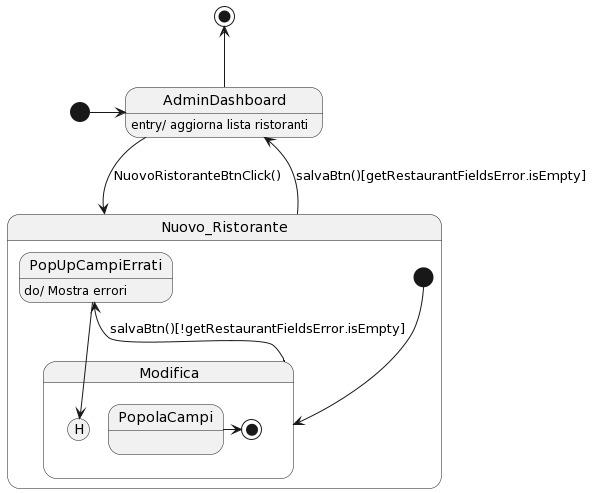
\includegraphics[scale=0.65]{assets/diagrammi/Statechart/aggiungiRistorante.png}
            \caption*{\textbf{Statechart} : aggiunta ristorante}\label{fig:Statechart_AddResturant}
        \end{figure}

    \subsubsection{Aggiungi piatto}
        \begin{figure}[H]
            \centering
            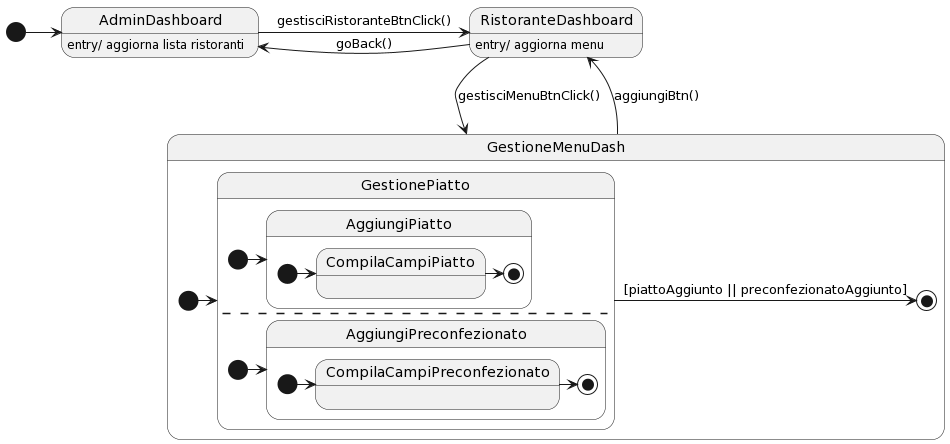
\includegraphics[scale=0.45]{assets/diagrammi/Statechart/aggiungiPiatto.png}
            \caption*{\textbf{Statechart} : aggiunta piatto}\label{fig:Statechart_AddPlate}
        \end{figure}

        \begin{figure}[H]
            \centering
            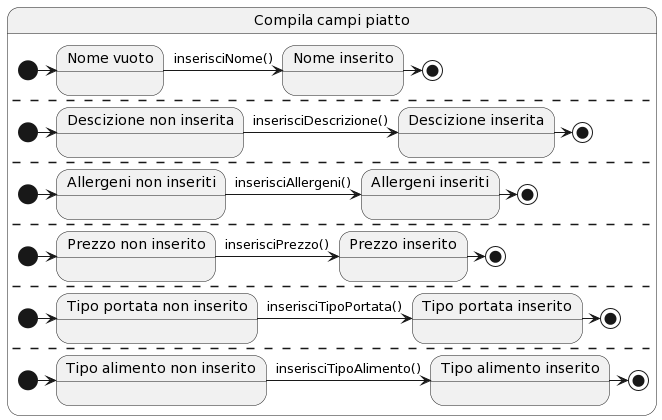
\includegraphics[scale=0.6]{assets/diagrammi/Statechart/compilaCampiPiatto.png}
            \caption*{\textbf{Statechart} : compilazione campi piatto non preconfezionato}\label{fig:Statechart_fieldPlate}
        \end{figure}

        \begin{figure}[H]
            \centering
            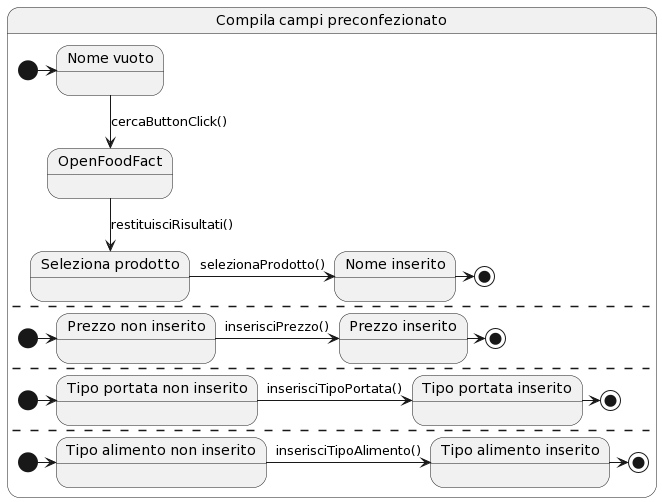
\includegraphics[scale=0.6]{assets/diagrammi/Statechart/compilaCampiPreconfezionato.png}
            \caption*{\textbf{Statechart} : compilazione campi piatto preconfezionato}\label{fig:Statechart_fieldPlate2}
        \end{figure}

    \subsubsection{Prendi ordine}
        \begin{figure}[H]
            \centering
            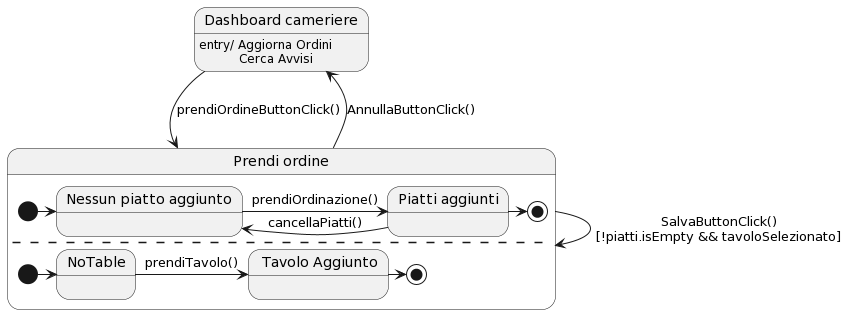
\includegraphics[scale=0.7]{assets/diagrammi/Statechart/prendiOrdine.png}
            \caption*{\textbf{Statechart} : Prendi ordinazione}\label{fig:Statechart_takeOrder}
        \end{figure}

    \subsubsection{Visualizza avvisi}
        \begin{figure}[H]
            \centering
            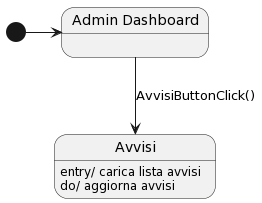
\includegraphics[scale=1]{assets/diagrammi/Statechart/visualizzaAvvisi.png}
            \caption*{\textbf{Statechart} : visualizzazione avvisi}\label{fig:Statechart_viewAdv}
        \end{figure}